\documentclass[10pt ]{article}

\usepackage{times}
\usepackage{epsfig}
\usepackage{graphicx}
\usepackage{amsmath}
\usepackage{amssymb}
\usepackage{amsthm}

\newtheorem{example}{Example}

\usepackage{tikz}
\usepackage{soul}
\usetikzlibrary{shapes.misc, positioning, shapes.geometric, arrows}
%\usepackage[a4paper,margin=1cm,landscape]{geometry}
\usetikzlibrary{positioning,shapes,shadows}


\tikzstyle{conv2d} = [rectangle, rounded corners, minimum width=4cm, minimum height=1cm,text centered, draw=black, fill=green!30]
\tikzstyle{bn} = [rectangle, rounded corners, minimum width=4cm, minimum height=1cm,text centered, draw=black, fill=red!30]
\tikzstyle{relu} = [rectangle, rounded corners, minimum width=4cm, minimum height=1cm,text centered, draw=black, fill=blue!30]
\tikzstyle{add} = [circle, radius=1cm,text centered, draw=black]
\tikzstyle{arrow} = [thick,->,>=stealth]
\tikzstyle{downsample} = [rectangle, minimum width=6cm, minimum height=4cm,text centered, draw=black, fill=yellow!30]
\tikzstyle{maxpool} = [rectangle, rounded corners, minimum width=4cm, minimum height=1cm,text centered, draw=black, fill=gray!30]

\tikzstyle{btds} = [rectangle, rounded corners, minimum width=4cm, minimum height=1cm,text centered, draw=black, fill=orange!30]

\tikzstyle{btnods} = [rectangle, rounded corners, minimum width=4cm, minimum height=1cm,text centered, draw=black, fill=violet!30]

\def\ttx{1.4}

\setcounter{page}{1}
\begin{document}

\title{Statistical Notes}

\author{Mohsen Kiskani}

\maketitle

%\begin{abstract}
%\end{abstract}

\section{Bayesian Inference}

We have a high dimensional parameter vector $\theta$ with a prior probability distribution $p(\theta)$. We want to see how our data is related to the parameters now that we have observed the data. In other words, we want to find $p(\theta | y_{1:N})$. We have,
\begin{align}
p(\theta | y_{1:N}) = \frac{ p(y_{1:N} | \theta) p(\theta)}{p(y_{1:N})}
\label{eq_bayesian_inference}
\end{align}
where $p(y_{1:N})$ is called {\em evidence}. Here are the steps for Bayesian inference:
\begin{enumerate}
\item Build a model, choose a {\em prior} $p(\theta)$ and a {\em likelihood} $p(y_{1:N} | \theta)$.
\item Compute the {\em posterior} using Bayes rule in equation \eqref{eq_bayesian_inference}.
\item Report a summary, e.g. posterior mean or (co)variance.
\end{enumerate}
There are many issues with this model. One of them is to find a good model for prior and likelihood. The other one, is the computational challenge in computing steps 2 and 3 since typically there is no closed form and it is hard to compute high dimensional integrations.
We only started with the models for prior and likelihood and we need to gather any other thing from this. Hence we need to compute the marginal distribution of evidence by the integrating the joint distribution using the following high dimensional integration which is often hard to compute,
\begin{align}
p(y_{1:N}) = \int p(y_{1:N} ; \theta) \mathrm{d}\theta
\label{eq_evidence}
\end{align}

\section{Monte Carlo methods}
These are approximate Bayesian inference techniques. Here is a little summary of some sampling techniques. 

\subsection{Importance Sampling}
Assume that we have a probability distribution $P(\mathbf{x})$ and we want to find the expected value of a function $\phi(\mathbf{x})$ based on this probability distribution.
\begin{align}
\Phi = \int P(x) \phi(x) \mathrm{d}x.
\label{eq_importance_sampling_E}
\end{align}
In general $\mathbf{x}$ can be a multi-dimensional vector but for illustrative purposes, we only consider a one dimensional density $P(x)$. We can evaluate this density at any chosen point $x$ at least to within a multiplicative constant; thus we can evaluate $P^*(x)$ such that 
\begin{align}
P(x) = \frac{P^*(x)}{Z}.
\label{eq_importance_sampling}
\end{align}
But $P(x)$ is too complicated a function for us to be able to sample from it directly e.g. $P(x)$ is a complicated density function like $\exp(0.4(x-0.4)^2-0.08x^4)$. Assume that $Q(x)$ is a simpler density function from which we can generate samples and which we can evaluate to within a multiplicative constant. That is, we can evaluate $Q^*(x)$ where, 
\begin{align}
Q(x) = \frac{Q^*(x)}{Z_Q}.
\label{eq_importance_sampling_Q}
\end{align}
In importance sampling, we generate $R$ samples $\{ x^r \}_{r=1}^R$ from $Q(x)$. If these points were samples from $P(x$) then we could estimate $\Phi$ as
\begin{align}
\hat{\Phi} = \frac{1}{R} \sum_{r=1}^R \phi(x^r).
\label{eq_importance_sampling_original_px}
\end{align}
 But when we generate samples from $Q$, values of $x$ where  $Q(x)$ is greater than $P(x)$ will be over-represented in this estimator, and points where $Q(x)$ is less than $P(x)$ will be under-represented. To take into account the fact that we have sampled from the wrong distribution, we introduce weights
\begin{align}
w_r = \frac{P^*(x^r)}{Q^*(x^r)},
\label{eq_importance_sampling_weights}
\end{align} 
which we use to adjust the {\em importance} of each point in our estimator thus:
 \begin{align}
\hat{\Phi} =  \frac{\sum_{r=1}^R w_r\phi(x^r)}{\sum_{r=1}^R w_r}.
\label{eq_importance_sampling_weights_applied}
\end{align}
We can prove that, if $Q(x)$ is non-zero for all $x$ where $P(x)$ is non-zero, the estimator $\hat{\Phi}$ converges to $\Phi$, the mean value of $\phi(x)$, as $R$ increases.  This is not necessarily an unbiased estimator but bias rapidly decreases with $R$. It is asymptotically unbiased.

A practical difficulty with importance sampling is that it is hard to estimate how reliable the estimator $\hat{\Phi}$ is. The variance of the estimator is unknown beforehand, because it depends on an integral over $x$ of a function involving $P^*(x)$. And the variance of $\hat{\Phi}$ is hard to estimate, because the empirical variances of the quantities $w_r$ and $w_r \phi(x^r)$ are not necessarily a good guide to the true variances of the numerator and denominator in equation \eqref{eq_importance_sampling_weights_applied}. If the proposal density $Q(x)$ is small in a region where $|\phi(x)P^*(x)|$ is large then it is quite possible, even after many points $x^r$ have been generated, that none of them will have fallen in that region. In this case the estimate of $\Phi$ would be drastically wrong, and there would be no indication in the empirical variance that the true variance of the estimator $\hat{\Phi}$ is large.

Importance sampling in high dimensions often suffers from two difficulties. First, we need to obtain samples that lie in the typical set of $P$, and this may take a long time unless $Q$ is a good approximation to $P$. Second, even if we obtain samples in the typical set, the weights associated with those samples are likely to vary by large factors, because the probabilities of points in a typical set, although similar to each other, still differ by factors of order $\exp(\sqrt{N})$, so the weights will too, unless $Q$ is a near-perfect approximation to $P$. This is a main disadvantage of importance sampling. 

%If the probability distribution $p(x)$ is exactly known (as opposed to up to a constant factor), then the following estimator can be used to estimated $\Phi$,
%\begin{align}
%\tilde{\Phi} =  \frac{1}{R}\sum_{r=1}^R w_r\phi(x^r).
%\label{eq_importance_sampling_weights_applied}
%\end{align}
%$\tilde{\Phi}$ also converges to $\Phi$ as $R \to \infty$.

\subsection{Rejection Sampling}

Refer to page 364 in \cite{mackay2003information}. Similar to importance sampling, rejection sampling will work best if $Q$ is a good approximation to $P$. If $Q$ is very different from $P$ then, for $c Q$ to exceed $P$ everywhere, $c$ will necessarily have to be large and the frequency of rejection will be large.

\section{Markov Chain Monte Carlo (MCMC) methods}
It's a very widely used technique since it is eventually accurate if you run it long enough but it is slow. It finds some approximation to the posterior and then finds it's mean and it's variance as approximate means and variances for our exact posterior. 

\subsection{The Metropolis–Hastings algorithm}

Importance sampling and rejection sampling work well only if the proposal density $Q(x)$ is similar to $P(x)$. In large and complex problems it is difficult to create a single density $Q(x)$ that has this property. The Metropolis–Hastings algorithm instead makes use of a proposal density $Q$ which depends on the current state $x^t$. The density $Q(x^{\prime};x^t)$ might be a simple distribution such as a Gaussian centered on the current $x^t$. The proposal density $Q(x^{\prime};x^t)$ can be any fixed density from which we can draw samples. In contrast to importance sampling and rejection sampling, it is not necessary that $Q(x^{\prime};x^t)$ look at all similar to $P(x)$ in order for the algorithm to be practically useful. As before, we assume that we can evaluate $P^*(x)$ for any $x$. A tentative new state $x^{\prime}$ is generated from the proposal density $Q(x^{\prime};x^t)$. To decide whether to accept the new state, we compute the quantity 
\begin{align}
a = \frac{ P^*(x^{\prime}) Q(x^t;x^{\prime})}{ P^*(x^t) Q(x^{\prime};x^t)}
\label{eq_metropolis_hasting_1}
\end{align}
If $a \ge 1$ then the new state is accepted. Otherwise, the new state is accepted with probability $a$. If the step is accepted, we set $x^{t+1} = x^{\prime}$. If the step is rejected, then we set $x^{t+1} = x^{t}$. Note the difference from rejection sampling: in rejection sampling, rejected points are discarded and have no influence on the list of samples $\{x^r\}$ that we collected. Here, a rejection causes the current state to be written again onto the list. Note that a Metropolis–Hastings simulation iterations does not produce independent samples from the target distribution $P$. The samples are dependent. The Metropolis method is an example of a Markov chain Monte Carlo method (abbreviated MCMC). In contrast to rejection sampling, where the accepted points $\{x^r\}$ are independent samples from the desired distribution, Markov chain Monte Carlo methods involve a Markov process in which a sequence of states $\{x^t\}$ is generated, each sample $x^t$ having a probability distribution that depends on the previous value, $x^{t-1}$. Since successive samples are dependent, the Markov chain may have to be run for a considerable time in order to generate samples that are effectively independent samples from $P$. 

Just as it was difficult to estimate the variance of an importance sampling estimator, so it is difficult to assess whether a Markov chain Monte Carlo method has `converged’, and to quantify how long one has to wait to obtain samples that are effectively independent samples from $P$.

To compute the acceptance probability, we need to be able to compute the probability ratios $\frac{P(x^{\prime})}{P(x^t)}$ and $\frac{Q(x^t;x^{\prime})}{Q(x^{\prime};x^t)}$. If the proposal density is a simple symmetrical density such as a Gaussian centred on the current point, then the latter factor is unity, and the Metropolis–Hastings method simply involves comparing the value of the target density at the two points. This special case is sometimes called the Metropolis method.

\section{Variational Methods}

In these methods, just as the Monte Carlo methods, the assumption is that there is a nasty probability distribution $P(x) = \frac{1}{Z} P^{\star}(x) =  \frac{1}{Z}  \exp(-E(x))$ for which calculating $P^{\star}(x) $ and $E(x)$ is easy but not quite simple enough to be able to answer interesting questions. In variational methods, the idea is to approximate $P(x)$ by a simpler distribution $Q(x;\theta)$ and adjust $\theta$ to get the best approximation to $P$. Then, approximate $\sum_x \phi(x) P(x)$ by $\sum_x \phi(x) Q(x; \theta^{\star})$. This way, as opposed to Monte Carlo methods, we are getting away with introducing extra random numbers in addition to the data that we gathered to do inference on. We use the KL divergence metric but the question is which of the following metrics should we use,
\begin{align}
\label{kl_formula_1}
D_{\mathrm{KL}}(P || Q) &=  \sum_{x} P(x)  \log \left( \frac{P(x)}{Q(x)}\right) \\
D_{\mathrm{KL}}(Q || P) &=  \sum_{x} Q(x)  \log \left( \frac{Q(x)}{P(x)}\right) 
\label{kl_formula_2}
\end{align}
Notice that \eqref{kl_formula_2} is easier to calculate compared to \eqref{kl_formula_1} since it involves expectations over a simpler probability distribution, i.e. $Q$. We have
\begin{align}
D_{\mathrm{KL}}(Q || P) &=  \sum_{x} Q(x)  \log \left( \frac{Q(x)}{P(x)}\right) = \sum_{x} Q(x) E(x) + \ln(Z) - H_Q(x).
\label{kl_formula_3}
\end{align}
Hence, to minimize $D_{\mathrm{KL}}(Q || P)$, it is enough to minimize the {\em variational free energy} defined as 
\begin{align}
\tilde{F}(\theta) &=  \sum_{x} Q(x; \theta) E(x)  - H_Q(x) \nonumber \\
&= \sum_{x} Q(x; \theta) E(x)  - \sum_{x}  Q(x; \theta) \ln \left( \frac{1}{Q(x; \theta)} \right).
\label{eq_var_free_energy}
\end{align}
Variatial free energy is lower bounded by $\tilde{F}(\theta) \ge - \ln (Z)$ so if we succeed in minimizing the variational free energy, we will have also minimized the KL distance between $Q$ and $P$ and the objective function that pops out of that minimization if we can evaluate the variational free energy at the optimum, then we get a bound on $\ln(Z)$.

\section{Approximate Bayesian Inference}
\subsection{MCMC based methods.}
These are the MCMC methods explained earlier. 

\subsection{Variational Bayes}
Can we use some form of optimization for inference? These methods try to solve the Bayesian inference problem using an approximation approach to find a good approximation $q^{\star}$. Assume that we have a space of {\em NICE} distributions out there for which we can compute the mean and the covariance fairly easily as we cannot easily calculate means and variances for $p(\theta | y)$. 
\begin{figure}[h]
\center
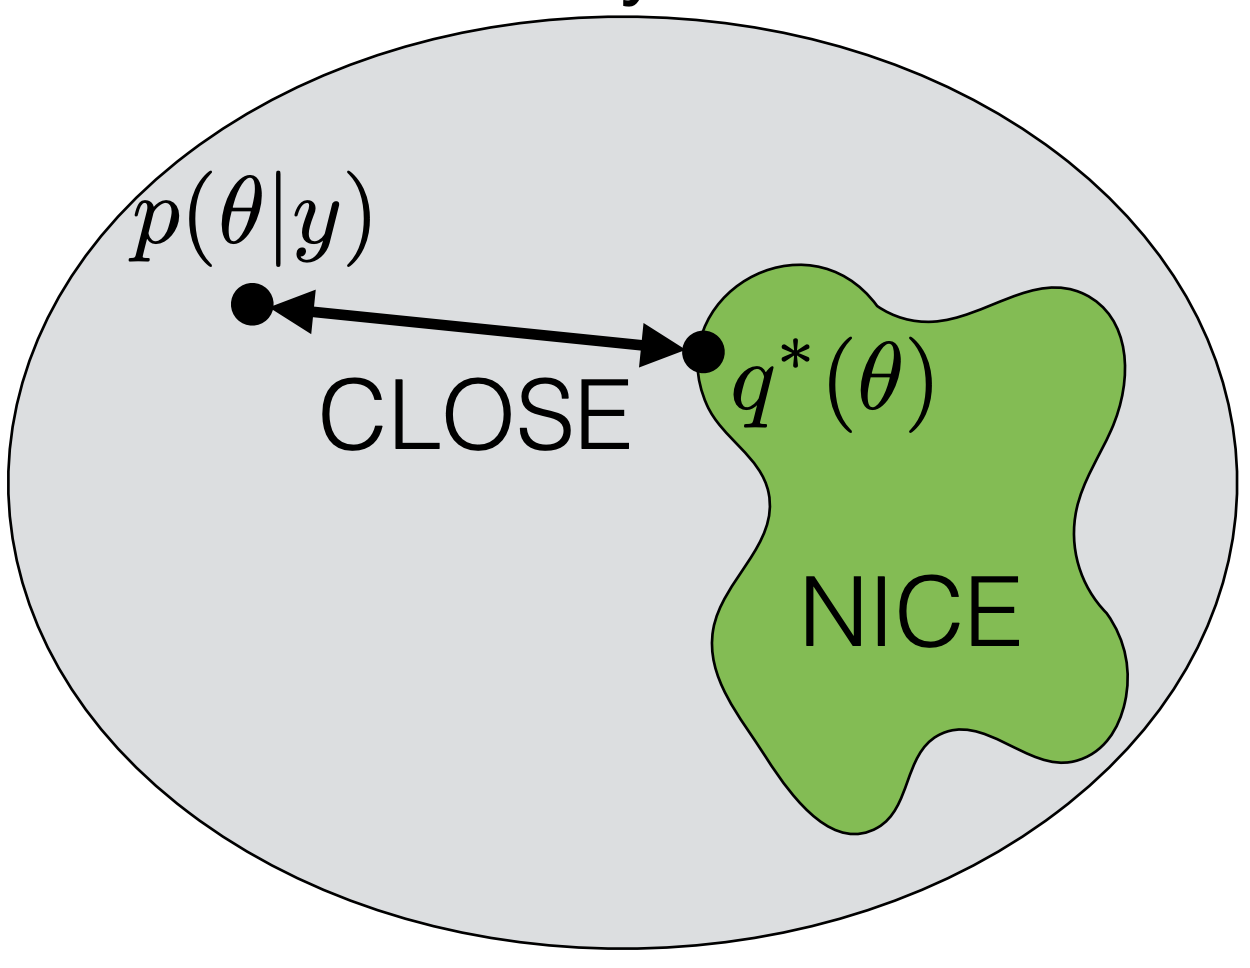
\includegraphics[scale=0.3]{close.png}
\end{figure}
The approach is to approximate $p(\theta | y)$ with the closest distribution in the NICE set. This is the goal of our optimization problem. 
\begin{align}
q^{\star} &= \mathrm{argmin}_{q \in Q} f(q(.), p(.|y))
\label{eq_find_min_q}
\end{align}
The measure of closeness $f(.)$ in Variational Bayes (VB) is KL divergence which makes the optimization problem much easier. 
\begin{align}
f(\theta) = \mathrm{KL}(q(\theta), p(\theta|y)) = \int q(\theta) \log \left(\frac{q(\theta) }{p(\theta | y)} \right) \mathrm{d}\theta
\label{eq_kl_eq}
\end{align}
This is not an actual distance as opposed to metrics like Wasserstein or total variation since it is not symmetric. This is a divergence as opposed to a distance. One reason for choosing it is that it is very fast and practical and widely used.  It is not possible to simply minimize the equation \eqref{eq_kl_eq} as it involves the knowledge of the exact posterior $p(\theta | y)$. This is not a problem unique to KL divergence but it is a problem for any metric. How can we optimize the problem and choose the closest distribution to a distribution that we don't know?!  We can do a little algebraic manipulation to write, 
\begin{align}
f(\theta) &= \mathrm{KL}(q(\theta), p(\theta|y)) = \int q(\theta) \log \left(\frac{q(\theta) }{p(\theta | y)} \right) \mathrm{d}\theta = \int q(\theta) \log \left(\frac{q(\theta) p(y)}{p(\theta , y)} \right) \mathrm{d}\theta \nonumber \\
&= \log(p(y)) - \int q(\theta) \log \left(\frac{p(\theta , y)}{q(\theta)} \right) \mathrm{d}\theta
\label{eq_kl_eq2}
\end{align}
The first term in equation \eqref{eq_kl_eq2} is not important as we want to minimize the KL divergence over $q$ and we can ignore this term. The second term also contains only things that we know since $p(\theta, y)$ is simply the product of the prior and likelihood so we have a hope of being able to optimize this. The second term in the right hand side of equation \eqref{eq_kl_eq2} is called \textbf{Evidence Lower Bound (ELBO)}. Since the KL divergence is always greater than or equal to zero and it's equal to zero exactly when the inputs are the same, we have 
\begin{align}
\log(p(y)) \ge \mathrm{ELBO} =  \int q(\theta) \log \left(\frac{p(\theta , y)}{q(\theta)} \right) \mathrm{d}\theta.
\label{eq_elbo}
\end{align}
Equation \eqref{eq_elbo} explains the name ELBO but more importantly, this equation shows that finding $q^{\star}$ to be the minimizer of the KL is exactly equivalent to finding $q^{\star}$ to be the maximizer of ELBO, 
\begin{align}
q^{\star} &= \mathrm{argmin}_{q \in Q} \mathrm{KL}(q(.), p(.|y))  \Leftrightarrow q^{\star} = \mathrm{argmax}_{q \in Q}  \mathrm{ELBO}.
\label{eq_elbo_equivalence}
\end{align}
We did not make any any assumptions or approximations. This is essentially the exact same problem. This is the main reason that KL divergence is used in VB as it is giving us a way to solve the optimization problem that we are interested to solve, in a very nice way using another optimization problem. In it's original form the integral is over the exact posterior which we don't know. 

Now, back to the original problem, what do we mean by a NICE distribution? We were trying to report means and variances. The first type of distributions that help us in achieving this goal are low dimensional approximations. This motivates us to choose \textbf{ Mean Field Variational Bayes (MFVB)}  assumption. In MFVB, the assumption is that although the parameter vector $\theta$ may be very high dimensional but it breaks down into components $\theta_1, \dots, \theta_J$ which don't have to be one dimensional but we imagine that they are smaller and easier to deal with. Further, we assume that the approximating distribution factorizes over these components,
\begin{align}
Q_{MFVB} = \left\{q \colon q(\theta) = \prod_{j=1}^J q_j(\theta_j) \right\}.
\label{eq_mvfb_def}
\end{align}
The second assumption on these distributions is the \textbf{exponential family} assumption. In fact, when people use the term MFVB they are implicitly having the assumption of exponential families on the approximating distributions. It is important to emphasize that MFVB assumption is an assumption on the approximation and not an assumption on the model itself. 

Now, that we have a well-defined optimization problem, we can solve it in any way we want. {\em Coordinate decent} is an example of an optimization technique that could be used to solve this optimization problem. The following diagram shows where we are in this process.
\begin{figure}[h]
\center
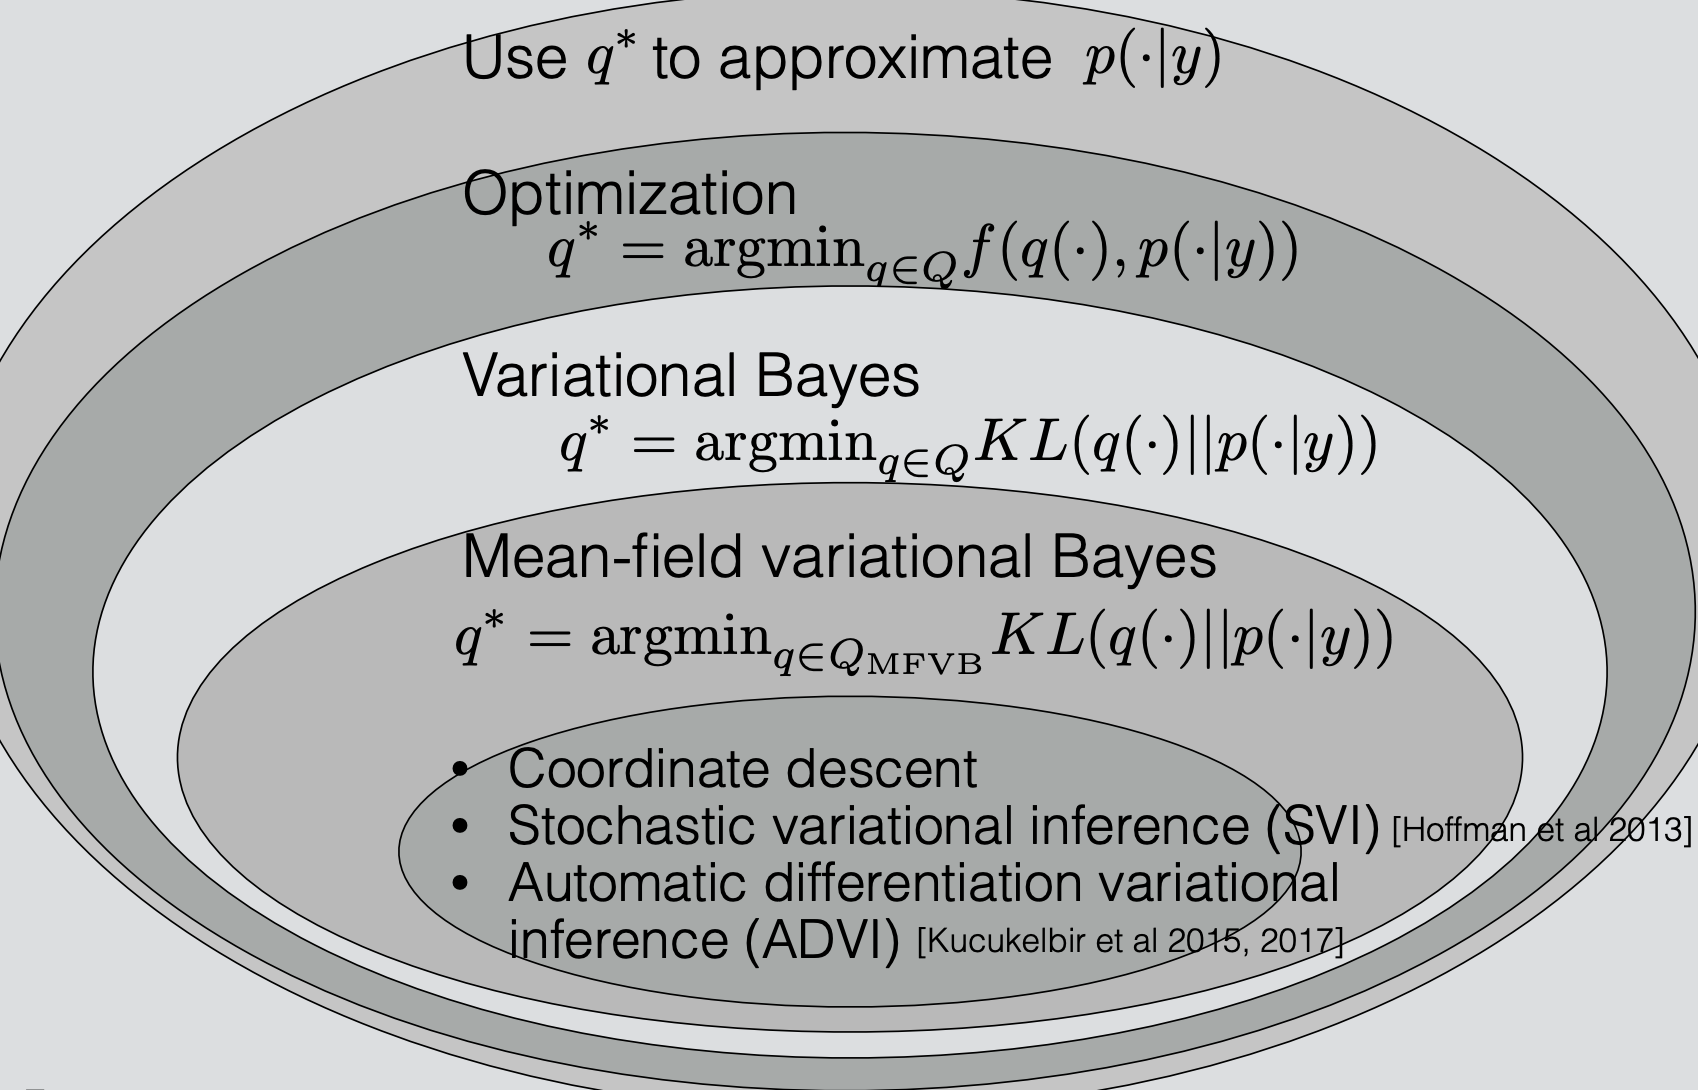
\includegraphics[scale=0.4]{subsets.png}
\end{figure}

If we replace equation \eqref{eq_mvfb_def} into the ELBO equation we have
\begin{align}
\mathrm{ELBO} &= \int_{\theta_1, \dots, \theta_J}  \prod_{j=1}^J q_j(\theta_j) \log \left(\frac{p(\theta, y) }{\prod_{j=1}^J q_j(\theta_j)} \right) \mathrm{d}\theta \nonumber \\
 &=  \int_{\theta_1, \dots, \theta_J}   \prod_{j=1}^J q_j(\theta_j) \left( \log(p(\theta, y)) - \sum_{j=1}^J \log \left( q_j (\theta_j)\right)\right) \mathrm{d}\theta  \nonumber \\
& = \int_{\theta_j}  q_j(\theta_j)   \left( \int_{\theta_i, i\neq j}   \prod_{i \neq j} q_i(\theta_i) \log(p(\theta, y)) \mathrm{d} \theta_{i, i \neq j} \right) \mathrm{d} \theta_j \nonumber \\
&\qquad - \int_{\theta_j}  q_j(\theta_j)  \log  \left(   q_j(\theta_j) \right) \mathrm{d} \theta_j + \mathrm{const} \nonumber \\
& = \int_{\theta_j} q_j ( \theta_j) \log \left( \tilde{p}_j(\theta, y) \right) \mathrm{d} \theta_j  - \int_{\theta_j}  q_j(\theta_j)  \log  \left(   q_j(\theta_j) \right) \mathrm{d} \theta_j + \mathrm{const},
\label{eq_elbo_mvfb}
\end{align}
Where the new distribution $\tilde{p}_j(\theta, y)$ is defined as
\begin{align}
\log \left( \tilde{p}_j(\theta, y) \right) &\triangleq \mathbb{E}_{i \neq j} \left[ \log \left( p(\theta, y) \right) \right] + \mathrm{const} \nonumber \\
&=  \int_{\theta_i, i\neq j}   \prod_{i \neq j} q_i(\theta_i) \log(p(\theta, y)) \mathrm{d} \theta_{i, i \neq j}  + \mathrm{const}
\label{eq_new_elbo_dist}
\end{align}
Now suppose we keep the $\{ q_{i \neq j} \}$ fixed and maximize ELBO in equation \eqref{eq_elbo_mvfb} with respect to all possible forms for the distribution $q_j(\theta_j)$. This is easily done by recognizing that  \eqref{eq_elbo_mvfb} is a negative KL divergence between $ \tilde{p}_j(\theta, y)  $ and $q_j(\theta_j)$. Thus maximizing \eqref{eq_elbo_mvfb}  is equivalent to minimizing the KL divergence between these two functions and the minimum KL divergence occurs when $ q_j(\theta_j) =  \tilde{p}_j(\theta, y) $. This gives us a general expression for the optimal solution $q_{j}^{\star} \left( \theta_j \right)$ as,
\begin{align}
\log \left( q_{j}^{\star} \left( \theta_j \right) \right) &= \mathbb{E}_{i \neq j} \left[ \log \left( p(\theta, y) \right) \right] + \mathrm{const}.
\label{eq_optimal_mvfb}
\end{align}
This equation says that the log of the optimal solution for factor $q_j$ is obtained simply by considering the log of the joint distribution over all hidden and visible variables and then taking the expectation with respect to all of the other factors $\{ q_i \}$ for $i \neq j$. 

The additive constant in \eqref{eq_optimal_mvfb} is set by normalizing the distribution $q_j(\theta_j)$. Thus if we take the exponential of both sides and normalize, we have
\begin{align}
 q_{j}^{\star} \left( \theta_j \right)  &=\frac{\exp \left( \mathbb{E}_{i \neq j} \left[ \log \left( p(\theta, y) \right) \right]  \right)}{\int_{\theta_i, i \neq j} \exp \left( \mathbb{E}_{i \neq j} \left[ \log \left( p(\theta, y) \right) \right]  \right) \mathrm{d} \theta_{i, i\neq j}}. 
\label{eq_optimal_mvfb_exp_form}
\end{align}
In practice, it is easier to work with equation \eqref{eq_optimal_mvfb} instead of equation \eqref{eq_optimal_mvfb_exp_form}. The set of equations given by \eqref{eq_optimal_mvfb} different values of $j$ represent a set of consistency conditions for the maximum of the lower bound subject to the factorization constraint. However, they do not represent an explicit solution because the expression on the right-hand side of \eqref{eq_optimal_mvfb} for the optimum $q_j(\theta_j)$ depends on expectations computed with respect to the other factors $q_j(\theta_j)$ for $i \neq j$. We will therefore seek a consistent solution by first initializing all of the factors $q_j(\theta_j)$ appropriately and then cycling through the factors and replacing each in turn with a revised estimate given by the right-hand side of \eqref{eq_optimal_mvfb} evaluated using the current estimates for all of the other factors. Convergence is guaranteed because bound is convex with respect to each of the factors.

\begin{example}
{\em We want to approximate a Gaussian distribution using factorized distributions.  Assume that we have $p( \mathbf{z} )= \mathcal{N}(  \mathbf{z}  | \mu, \Lambda^{-1})$ over two correlated variables $\mathbf{z}  = (z_1,z_2)$ in which the mean and precision have elements
\begin{align}
\mu = \begin{bmatrix}
\mu_1 \\ \mu_2
\end{bmatrix}, 
\qquad 
\Lambda = \begin{bmatrix}
\Lambda_{11} & \Lambda_{12} \\ \Lambda_{21} & \Lambda_{22} 
\end{bmatrix} 
\end{align}
where $ \Lambda_{12} = \Lambda_{21} $ due to the symmetry of the precision matrix. We wish to approximate this distribution using a factorized Gaussian of the form $q(\mathbf{z}) = q_1(z_1)q_2(z_2)$. We can use the equation \eqref{eq_optimal_mvfb} by considering that $y$ is nothing and $\mathbf{z} = \theta$. Using equation \eqref{eq_optimal_mvfb} to find an expression for the optimal factor $q_1^{\star}(z_1)$, on the right-hand side we only need to retain those terms that have some functional dependence on $z_1$ because all other terms can be absorbed into the normalization constant. We have,
\begin{align}
\log (q_1^{\star}(z_1)) &= \mathbb{E}_{z_2} \left[ \log \left( p(\mathbf{z}  ) \right) \right] + \mathrm{const} \nonumber \\
&= \mathbb{E}_{z_2} \left[ -\frac{1}{2} (z_1 - \mu_1)^2 \Lambda_{11} - (z_1 - \mu_1) \Lambda_{12} (z_2 - \mu_2)  \right] + \mathrm{const} \nonumber \\
&= -\frac{1}{2} z_1^2 \Lambda_{11}  + z_1 \mu_1 \Lambda_{11} - z_1 \Lambda_{12} (\mathbb{E}(z_2) -\mu_2) +  \mathrm{const}.
\label{eq_ex_1}
\end{align}
Observe that the right-hand side of this expression is a quadratic function of $z_1$, and so we can identify $q(z_1)$ as a Gaussian distribution. It is worth emphasizing that we did not assume that $q(z_i)$ is Gaussian, but rather we derived this result by variational optimization of the KL divergence over all possible distributions $q(z_i)$. Note also that we do not need to consider the additive constant in \eqref{eq_optimal_mvfb} explicitly because it represents the normalization constant that can be found at the end by inspection if required. Using the technique of completing the square, we can identify the mean and precision of this Gaussian, giving
\begin{align}
q_1^{\star}(z_1) &= \mathcal{N} (z_1 | m_1, \Lambda_{11}^{-1})
\label{eq_z1_derivation}
\end{align}
where
\begin{align}
m_1 = \mu_1 - \Lambda_{11}^{-1} \Lambda_{12} \left( \mathbb{E}(z_2) - \mu_2\right)
\label{eq_m1_derivation}
\end{align}
By symmetry $q_2^{\star}(z_2) $ is also Gaussian and can be written as
\begin{align}
q_2^{\star}(z_2) &= \mathcal{N} (z_2 | m_2, \Lambda_{22}^{-1})
\label{eq_z2_derivation}
\end{align}
where
\begin{align}
m_2 = \mu_2 - \Lambda_{22}^{-1} \Lambda_{21} \left( \mathbb{E}(z_1) - \mu_1\right)
\label{eq_m2_derivation}
\end{align}
Note that these solutions are coupled, so that $q^{\star}(z_1)$ depends on expectations computed with respect to $q^{\star}(z_2)$  and vice versa. In general, we address this by treating the variational solutions as re-estimation equations and cycling through the variables in turn updating them until some convergence criterion is satisfied. Here, however, we note that the problem is sufficiently simple that a closed form solution can be found. In particular, because $\mathbb{E}[z_1] = m_1$ and $\mathbb{E}[z_2] = m_2$, we see that the two equations are satisfied if we take $\mathbb{E}[z_1] = \mu_1$ and $\mathbb{E}[z_2] = \mu_2$, and it is easily shown that this is the only solution provided the distribution is nonsingular. 
}
\label{example_normal}
\end{example}

\begin{example}
{\em We have $N$ i.i.d observations $y = (y_1, \dots, y_N )$ and we assume that they are coming from a normal distribution $\mathcal{N}(\mu, \tau^{-1})$ where $\tau$ or precision  is the inverse of variance i.e., we assume that the likelihood function is normal. 
\begin{align}
p(y | \mu, \tau ) & = \left( \frac{\tau}{2 \pi }\right)^{\frac{N}{2}} \exp \left( -\frac{\tau}{2}  \sum_{i=1}^N (y_i - \mu)^2 \right)
\label{eq_gaussian_models}
\end{align}
We are interested in finding the posterior mean $\mu$ and precision $\tau$ distributions.  To complete our model, we have to also add a prior distribution. A particular conjugate prior that we can choose, is a gamma prior for the inverse variance or precision and a normal prior for $ \mu | \tau $  as follows, 
\begin{align}
p(\tau) &= \mathrm{Gamma}(\tau | a_0, b_0) = \frac{1}{\Gamma(a_0)} b_0^{a_0}{\tau^{a_0-1}} \exp(-{b_0}{\tau}). \\
p(\mu | \tau) & =    \mathcal{N}(\mu_0, (\lambda_0 \tau)^{-1}) = \sqrt{\frac{\lambda_0 \tau}{2 \pi}} \exp \left( -\frac{\lambda_0 \tau}{2} (\mu - \mu_0)^2\right).
\end{align}
 What we mean by conjugate is that if I have this prior and if I have this likelihood, I can calculate the posterior exactly without needing to do any approximations.  The posterior gets a form of Gaussian-Gamma distribution. This is good as it allows us to check the result of our VB approximation with the actual values of the posterior.  
 
Using MFVB assumption we can find the posteriors but notice that there is no MFVB assumption on the model and therefore $p(\mu, \tau|y) \neq f_1(\mu, y) f_2(\tau, y)$.  The MFVB assumption is as follows,
\begin{align}
q(\mu, \tau) = q_{\mu} (\mu) q_{\tau} (\tau).
\label{eq_mfvb_assumption_toy}
\end{align}
We can compute the ELBO as follows and then try to optimize it,
\begin{align}
\mathrm{ELBO} &= \int_{\mu} \int_{\tau} q_{\mu} (\mu) q_{\tau} (\tau) \log \left(  \frac{ p(y | \mu, \tau) p(\mu | \tau) p(\tau)}{q_{\mu} (\mu) q_{\tau} (\tau)} \right) \mathrm{d} \tau \mathrm{d}\mu.
\label{eq_derivations}
\end{align}
However, a simpler way is to use equation \eqref{eq_optimal_mvfb}. Using this equation we have
\begin{align}
\log \left( q^{\star}_{\mu} (\mu) \right) &= \mathbb{E}_{\tau} \left[ \log \left( p (y | \mu, \tau) \right) + \log(\mu | \tau) \right]  + \mathrm{const}.  
\label{eq_mvfb_normal_10}
\\
\log \left( q^{\star}_{\tau} (\tau) \right) &= \mathbb{E}_{\mu} \left[ \log \left( p (y | \mu, \tau) \right) + \log(\mu | \tau)  + \log (p(\tau))  \right] +  \mathrm{const}. 
\label{eq_mvfb_normal_11}
\end{align}
From equation \eqref{eq_mvfb_normal_10} we have
\begin{align}
\log \left( q_{\mu}^{\star}(\mu) \right) &=  -\frac{\mathbb{E}_{\tau}\left[  \tau \right]}{2}  \left( \sum_{i=1}^N (y_i - \mu)^2 + \lambda_0  (\mu -\mu_0)^2  \right) +  \mathrm{const},
\label{eq_mvfb_normal_2}
\end{align}
and from equation \eqref{eq_mvfb_normal_11} we have, 
\begin{align}
\log \left( q^{\star}_{\tau} (\tau) \right) &=  -\frac{\tau}{2} \mathbb{E}_{\mu}\left[  \sum_{i=1}^N (y_i - \mu)^2 + \lambda_0  (\mu -\mu_0)^2  \right] \nonumber \\
&\qquad + \left( a_0 + \frac{N-1}{2} \right) \log(\tau) - b_0 \tau +  \mathrm{const},
\label{eq_mvfb_normal_3}
\end{align}
By completing the square in equation \eqref{eq_mvfb_normal_2} over $\mu$ we can prove that $ q_{\mu}^{\star}(\mu)$ is a Gaussian distribution $\mathcal{N}(\mu | \mu_N, \lambda_N^{-1})$ with mean $\mu_N$ and precision $\lambda_N$ where 
\begin{align}
\mu_N &= \frac{ \mu_0 \lambda_0 + N \bar{y}}{\lambda_0 + N}.
\label{eq_mvfb_normal_41}
\\
\lambda_N &= \left( \lambda_0 + N \right) \mathbb{E}_{\tau} \left[ \tau \right].
\label{eq_mvfb_normal_42}
\end{align} 
 We can also verify that equation \eqref{eq_mvfb_normal_3} results in a gamma distribution $\mathrm{Gamma}(\tau | a_N, b_N)$ for $q^{\star}_{\tau} (\tau) $ where
\begin{align}
a_N &= a_0 + \frac{N+1}{2}
\label{eq_mvfb_normal_51} 
\\
b_N &= b_0 + \frac{1}{2} \mathbb{E}_{\mu} \left[ \sum_{i=1}^N (y_i - \mu)^2 + \lambda_0  (\mu -\mu_0)^2 \right]
\label{eq_mvfb_normal_52}
\end{align}

It should be emphasized that we did not assume these specific functional forms for the optimal distributions $q^{\star}_{\mu} (\mu)$and $q^{\star}_{\tau} (\tau)$. They arose naturally from the structure of the likelihood function and the corresponding conjugate priors. 

Notice that we have expressions for the optimal distributions $q^{\star}_{\mu} (\mu)$ and $q^{\star}_{\tau} (\tau)$ each of which depends on moments evaluated with respect to the other distribution. One approach to finding a solution is therefore to make an initial guess for, say, the moment $\mathbb{E}_{\tau} \left[ \tau \right]$ and use this to re-compute the distribution $q^{\star}_{\mu} (\mu)$ . Given this revised distribution we can then extract the required moments $\mathbb{E}_{\mu} \left[ \mu \right]$ and $\mathbb{E}_{\mu} \left[ \mu^2 \right]$, and use these to recompute the distribution $q^{\star}_{\tau} (\tau)$, and so on.

In general, we will need to use an iterative approach such as this in order to solve for the optimal MFVB posterior distribution. For the very simple example we are considering here, however, we can find an explicit solution by solving the simultaneous equations for the optimal factors $q^{\star}_{\mu} (\mu)$ and $q^{\star}_{\tau} (\tau)$. Before doing this, we can simplify these expressions by considering broad, noninformative priors in which $\mu_0 = a_0 = b_0 = \lambda_0 = 0$. Although these parameter settings correspond to improper priors, we see that the posterior distribution is still well defined. Using the standard result $\mathbb{E}_{\tau} [\tau] = a_N / b_N$ for the mean of a gamma distribution, together with \eqref{eq_mvfb_normal_51} and \eqref{eq_mvfb_normal_52}, we have
\begin{align}
\frac{1}{\mathbb{E}_{\tau} [\tau]} = \frac{1}{N+1} \mathbb{E}_{\mu} \left[ \sum_{i=1}^N (y_i -\mu)^2 \right] =  \frac{N}{N+1} \left( \bar{y^2}- 2 \bar{y}\mathbb{E}_{\mu} \left[\mu \right] +  \mathbb{E}_{\mu} \left[\mu^2 \right] \right).
\label{eq_mfvb_normal_6}
\end{align}
Now, using equations \eqref{eq_mvfb_normal_41} and \eqref{eq_mvfb_normal_42} and \eqref{eq_mfvb_normal_6} we have
\begin{align}
&\mathbb{E}_{\mu} \left[ \mu \right] = \bar{y} \\
\label{eq_mfvb_normal_71}
\\
&\mathbb{E}_{\mu} \left[ \mu^2 \right] = \bar{y^2} + \frac{1}{N \mathbb{E}_{\tau} \left[ \tau \right]} 
\label{eq_mfvb_normal_72}
\\
&\frac{1}{\mathbb{E}_{\tau} \left[ \tau \right]} = \bar{y^2} -\bar{y}^2 = \frac{1}{N} \sum_{i=1}^N (y_i - \bar{y})^2
\end{align}

}
\label{example_gauddian}
\end{example}

\subsection{Variational model comparison}

As well as performing inference over the hidden variables $\theta$, we may also wish to compare a set of candidate models, labeled by the index $m$, and having prior probabilities $p(m)$. Our goal is then to approximate the posterior probabilities $p(m|y)$, where $y$ is the observed data. This is a slightly more complex situation than what we considered before because different models may have different structure and indeed different dimensionality for the hidden variables $\theta$. We cannot therefore simply consider a factorized approximation $q(\theta)q(m)$, but must instead recognize that the posterior over $\theta$ must be conditioned on $m$, and so we must consider $q(\theta, m) = q(\theta|m)q(m)$. We can readily verify the following decomposition based on this variational distribution
\begin{align}
\log \left( p (y) \right) &=  \sum_{m} \sum_{\theta} q(\theta | m) q(m) \log \left( \frac{p(\theta, m, y)}{q(\theta | m ) q(m)}\right) \nonumber \\
&-  \sum_{m} \sum_{\theta} q(\theta | m) q(m) \log \left( \frac{p(\theta, m | y)}{q(\theta | m ) q(m)}\right).
\label{eq_vb_model_1}
\end{align}
The second term in \eqref{eq_vb_model_1} is the KL divergence $\mathrm{KL} ( q(\theta , m ), p(\theta, m |y))$ and is always positive. Hence, the first term is a lower bound on $\log \left( p (y) \right)$ and it will become equal to $\log \left( p (y) \right)$ when $q(\theta , m )$ becomes equal to $p(\theta, m |y))$. If we rename the lower bound term as 
\begin{align}
\mathcal{L}_m &\triangleq  \sum_{m} \sum_{\theta} q(\theta | m) q(m) \log \left( \frac{p(\theta, m, y)}{q(\theta | m ) q(m)}\right), 
\label{eq_vb_model_2}
\end{align}
then we can maximize $\mathcal{L}_m$ with respect to the distribution $q(m)$ using a Lagrange multiplier, with the result
\begin{align}
q(m) \propto p(m) \exp (\mathcal{L}_m).
\label{eq_vb_model_3}
\end{align}
However, if we maximize $\mathcal{L}_m$  with respect to the $q(\theta|m)$, we find that the solutions for different $m$ are coupled, as we expect because they are conditioned on $m$. We proceed instead by first optimizing each of the $q(\theta|m)$ individually by optimization of \eqref{eq_vb_model_2}, and then subsequently determining the $q(m)$ using \eqref{eq_vb_model_3}. After normalization the resulting values for $q(m)$ can be used for model selection or model averaging in the usual way.

\subsection{Variational mixture of Gaussians}
A Gaussian mixture distribution can be written as a linear superposition of Gaussians in the form
\begin{align}
p( y )= \sum_{k=1}^K \pi_k \mathcal{N} (y | \mu_k, \Sigma_k)
\label{eq_mog_def}
\end{align}
Let us introduce a $K$-dimensional binary random variable $\mathbf{z}$ having a 1-of-$K$ representation in which a particular element $z_k$ is equal to 1 and all other elements are equal to 0. The values of $z_k$ therefore satisfy $z_k \in \{0, 1\}$ and $ \sum_k z_k = 1$, and we see that there are $K$ possible states for the vector $\mathbf{z}$ according to which element is nonzero. We shall define the joint distribution $p(y, \mathbf{z})$ in terms of a marginal distribution $p(\mathbf{z})$ and a conditional distribution $p(y|\mathbf{z})$. The marginal distribution over $\mathbf{z}$ is specified in terms of the mixing coefficients $\pi_k$, such that
\begin{align}
p(z_k = 1 ) = \pi_k
\label{eq_mog_def_z}
\end{align}
where the parameters $\{\pi_k\}$ must be between 0 and 1 and they all should sum up to 1 in order to be valid probabilities. Because $\mathbf{z}$ uses a 1-of-$K$ representation, we can also write this distribution in the form
\begin{align}
p ( \mathbf{z}) = \prod_{k=1}^K \pi_k^{z_k}
\label{eq_mog_dist_z}
\end{align}
Similarly, the conditional distribution of $y$ given a particular value for $\mathbf{z}$ is a Gaussian
\begin{align}
p (y | z_k =1 ) = \mathcal{N}(y | \mu_k, \Sigma_k)
\label{eq_mog_dist_y_cond_z}
\end{align}
which can also be written in the form
\begin{align}
p (y | \mathbf{z}) =\prod_{k=1}^K \left( \mathcal{N}(y | \mu_k, \Sigma_k) \right)^{z_k}
\label{eq_mog_dist_y_cond_z_all}
\end{align}
The joint distribution is given by $p(\mathbf{z})p(y|\mathbf{z})$, and the marginal distribution of $y$ is then obtained by summing the joint distribution over all possible states of $\mathbf{z}$ to give
\begin{align}
p( y )= \sum_{\mathbf{z}}  p(\mathbf{z})p(y|\mathbf{z})= \sum_{k=1}^K \pi_k \mathcal{N} (y | \mu_k, \Sigma_k)
\label{eq_mog_marginal_def}
\end{align}
We have therefore found an equivalent formulation of the Gaussian mixture involving an explicit latent variable. It might seem that we have not gained much by doing so. However, we are now able to work with the joint distribution $p(y, \mathbf{z})$ instead of the marginal distribution $p(y)$, and this will lead to significant simplifications, most notably through the use of the expectation-maximization (EM) algorithm and the MFVB techniques. 

For each observation $y_i$ we have a corresponding latent variable $\mathbf{z}_n$ comprising a 1-of-$K$ binary vector with elements $z_{n k}$ for $k = 1, \dots ,K$. We denote the observed data set by $\mathbf{Y} = \{y_1, \dots ,y_N\}$, and similarly we denote the latent variables by $\mathbf{Z} = \{\mathbf{z}_1, \dots, \mathbf{z}_N\}$. We can write down the conditional distribution of $\mathbf{Z}$, given the mixing coefficients $\pi$, in the form
\begin{align}
p ( \mathbf{Z} | \pi) =\prod_{n=1}^N \prod_{k=1}^K \pi_k^{z_{n k}}.
\label{eq_mog_dist_z_modified}
\end{align}
Similarly, the conditional distribution of the observed data vectors, given the latent variables and the component parameters can be written as 
\begin{align}
p ( \mathbf{Y} |  \mathbf{Z} , \mu, \Lambda) =\prod_{n=1}^N \prod_{k=1}^K \mathcal{N} (y_n | \mu_k, \Lambda_k^{-1})^{z_{n k}}. 
\label{eq_mog_dist_cond_z_modified}
\end{align}
Next we introduce priors over the parameters $\mu, \Lambda, \pi$. The analysis is considerably simplified if we use conjugate prior distributions. We therefore choose a {\em Dirichlet distribution} over the mixing coefficients $\pi$.
\begin{align}
p(\pi | \alpha_0 ) = \mathrm{Dir} ( \pi | \alpha_0 ) = C(\alpha_0) \prod_{k=1}^K \pi_k^{\alpha_0 - 1}
\label{eq_dirichlet_dist}
\end{align}
where by symmetry we have chosen the same parameter $\alpha_0$ for each of the components, and $ C(\alpha_0)$ is the normalization constant for the Dirichlet distribution defined as 
\begin{align}
C(\alpha_0) = \frac{\Gamma (K \alpha_0) }{\left( \Gamma (\alpha_0) \right)^K}.
\label{eq_define_c_alpha_0}
\end{align}
The parameter $\alpha_0$ can be interpreted as the effective prior number of observations associated with each component of the mixture. If the value of $\alpha_0$ is small, then the posterior distribution will be influenced primarily by the data rather than by the prior. Similarly, we introduce an independent Gaussian-Wishart prior governing the mean and precision of each Gaussian component, given by
\begin{align}
p (\mu, \Lambda) &= p(\mu | \Lambda) p (\Lambda) \nonumber \\
&= \prod_{k=1}^K \mathcal{N} (\mu_k | m_0, (\beta_0 \Lambda_k)^{-1}) \mathcal{W} (\Lambda_k | w_0, \nu_0),
\label{eq_mog_prior_gauusian_wishart}
\end{align}
because this represents the conjugate prior distribution when both the mean and precision are unknown. Typically we would choose $m_0 = 0$ by symmetry. In order to formulate a variational treatment of this model, we next write down the joint distribution of all of the random variables, which is given by
\begin{align}
p(\mathbf{Y}, \mathbf{Z}, \pi, \mu, \Lambda) = p(\mathbf{Y}|\mathbf{Z}, \mu, \Lambda)p(\mathbf{Z}|\pi) p(\pi) p(\mu | \Lambda) p (\Lambda) 
\label{eq_mog_mfvb_joint_all}
\end{align}
We now consider a variational distribution which factorizes between the latent variables and the parameters so that
\begin{align}
q(\mathbf{Z}, \pi, \mu, \Lambda) = q(\mathbf{Z}) q(\pi, \mu, \Lambda) 
\label{eq_mog_q_def}
\end{align}
It is remarkable that this is the only assumption that we need to make in order to obtain a tractable practical solution to our Bayesian mixture model. In particular, the functional form of the factors $ q(\mathbf{Z}) $ and $ q(\pi, \mu, \Lambda) $ will be determined automatically by optimization of the variational distribution. Note that we are omitting the subscripts on the q distributions, much as we do with the $p$ distributions in \eqref{eq_mog_mfvb_joint_all}, and are relying on the arguments to distinguish the different distributions.

The corresponding sequential update equations for these factors can be easily derived by making use of the general result \eqref{eq_optimal_mvfb}. Let us consider the derivation of the update equation for the factor $q(\mathbf{Z})$. Using \eqref{eq_mog_mfvb_joint_all}, the log of the optimized factor is given by
\begin{align}
\log \left( q^{\star}(\mathbf{Z}) \right) &= \mathbb{E}_{\pi, \mu, \Lambda} \left[ \log \left(p(\mathbf{Y}, \mathbf{Z}, \pi, \mu, \Lambda) \right) \right] + \mathrm{const.} \nonumber \\
&= \mathbb{E}_{\pi, \mu, \Lambda} \left[ \log \left(p(\mathbf{Y}|\mathbf{Z}, \mu, \Lambda)p(\mathbf{Z}|\pi) p(\pi) p(\mu | \Lambda) p (\Lambda) \right) \right] + \mathrm{const.}
\label{eq_mfvb_mog_qz}
\end{align}
Note that we are only interested in the functional dependence of the right-hand side on the variable $\mathbf{Z}$. Thus any terms that do not depend on $\mathbf{Z}$ can be absorbed into the additive normalization constant, giving
\begin{align}
\log \left( q^{\star}(\mathbf{Z}) \right) &= \mathbb{E}_{\mu, \Lambda}  \left[ \log \left(p(\mathbf{Y}|\mathbf{Z}, \mu, \Lambda) \right) \right] + \mathbb{E}_{\pi} \left[ \log (p(\mathbf{Z}|\pi )) \right] + \mathrm{const.}
\label{eq_mfvb_mog_qz_2}
\end{align}
Similarly using \eqref{eq_optimal_mvfb} we have 
\begin{align}
\log \left( q^{\star}(\pi, \mu, \Lambda) \right)&=  \mathbb{E}_{\mathbf{Z}}  \left[ \log \left(p(\mathbf{Y}, \mathbf{Z}, \pi, \mu, \Lambda) \right) \right] + \mathrm{const.} \nonumber \\
&= \mathbb{E}_{\mathbf{Z}} \left[ \log \left(p(\mathbf{Y}|\mathbf{Z}, \mu, \Lambda)p(\mathbf{Z}|\pi) p(\pi) p(\mu | \Lambda) p (\Lambda) \right) \right] + \mathrm{const.}
\label{eq_mfvb_mog_qz_2}
\end{align}
Please continue the rest from \cite{bishop2006pattern}.



\bibliographystyle{plain}
\bibliography{summary_refs}
\end{document}


Substituting for the two conditional distributions on the right-hand side, and again absorbing any terms that are independent of $\mathbf{Z}$ into the additive constant, we have


 First, let's compute the exact posterior. 
\begin{align}	
\ln \left( p(y | \mu, \sigma^2) \right) = -N \ln (\sqrt{2 \pi} \sigma) - \frac{1}{2 \sigma^2} \left[ N (\mu - \bar{y})^2 +S\right]
\end{align}
where 
\begin{align}
\bar{y} &= \frac{1}{N} \sum_{i=1}^N y_i  \\
S &= \sum_{i=1}^N (y_i-\bar{y})^2
\label{eq_def_S_x_bar}
\end{align}

\begin{figure}[h]
\center
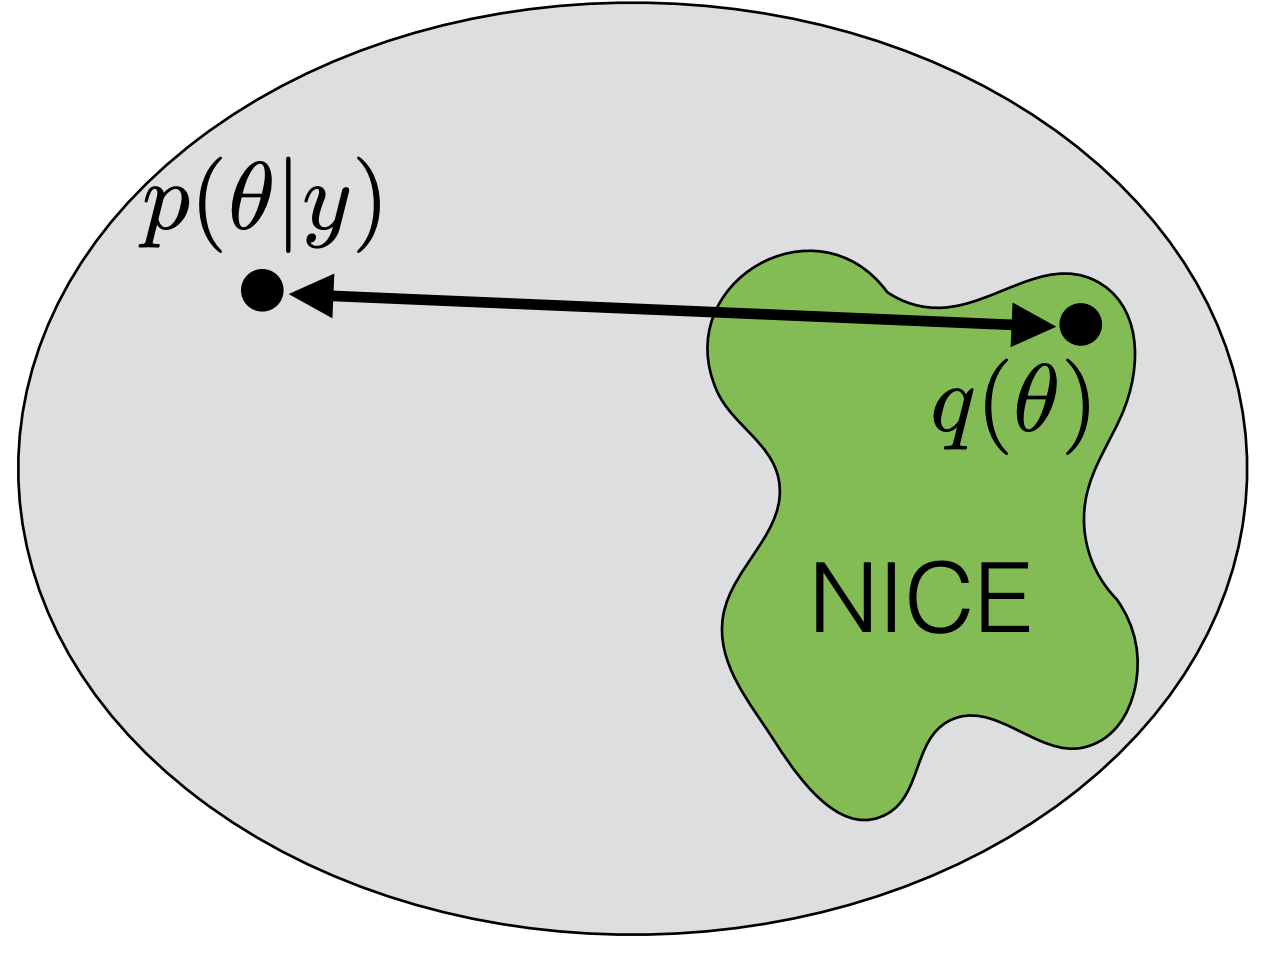
\includegraphics[scale=0.3]{nice.png}
\end{figure}

\begin{proof}
d
\label{proof_ex_1}
\end{proof}